\chapter{Basi di dati relazionali distribuite}
\begin{definizione}[\textbf{DDBMS}]
    Un \textbf{DBMS distribuito eterogeneo autonomo} è in generale una
    federazione di DBMS che collaborano per fornire accesso ai dati con livelli
    di trasparenza.
\end{definizione}
Con il termine trasparenza si intende la capacità di un sistema di
nascondere i dettagli di implementazione e di gestione dei dati, fornendo
all'utente una visione unificata e coerente del sistema.
\paragraph{Autonomia} L'autonomia fa riferimento al grado di indipendenza tra i
nodi. Possiamo distinguere diversi livelli di autonomia:
\begin{itemize}
    \item \textbf{Autonomia di progetto}: ogni nodo ha un proprio modello dei
          dati e di gestione delle transizioni.
    \item \textbf{Autonomia di condivisione}: ogni nodo sceglie la porzione di
          dati da condividere con gli altri nodi.
    \item \textbf{Autonomia di esecuzione}: ogni nodo sceglie in che modo eseguire
          le transazioni.
\end{itemize}
Partendo da questa classificazione possiamo definire diversi tipi di DBMS autonomi:
\begin{itemize}
    \item \textbf{DBMS Strettamente integrati}: in questo caso non c'è nessuna
          autonomia, i dati sono logicamente centralizzati ed esiste un unico
          data manager responsabile delle transazioni applicative. I data
          manager locali non operano in maniera autonoma.
    \item \textbf{Semi - autonomi}: ogni data manager è autonomo ma partecipa
          alle transazioni globali. Una parte dei dati è condivisa e richiedono
          modifiche architetturali per poter far parte della federazione.
    \item \textbf{Totalmente autonomi} (peer - to - peer): ogni DBMS lavora in
          completa autonomia ed è inconsapevole dell'esistenza degli altri.
\end{itemize}
\paragraph{Distribuzione} La distribuzione dei dati può avvenire in diversi
modi:
\begin{itemize}
    \item Distribuzione client - server: i dati sono distribuiti su più server
          e i client accedono ai dati attraverso le richieste fatte ai server.
          I server forniscono la gestione dei dati, mentre i client forniscono
          l'applicativo e la presentazione.
    \item Distribuzione peer - to - peer: i dati sono distribuiti su più nodi
          e ogni nodo può essere sia client che server. Ogni nodo è autonomo
          e può eseguire transazioni locali.
    \item Nessuna distribuzione: i dati sono centralizzati
\end{itemize}
\paragraph{Eterogeneità} L'eterogeneità si riferisce alla diversità dei DBMS
che compongono la federazione. Questa diversità può essere di diversi tipi:
\begin{itemize}
    \item \textbf{Linguaggio di interrogazione}: i DBMS possono utilizzare
          linguaggi di interrogazione diversi.
    \item \textbf{Modello dei dati}: i DBMS possono utilizzare modelli di dati
          diversi.
    \item \textbf{Sistema di gestione delle transazioni}: i DBMS possono utilizzare
          sistemi di gestione delle transazioni diversi.
    \item \textbf{Schema concettuale}: i DBMS possono avere schemi concettuali
          diversi.
\end{itemize}
Sviluppando una o più di queste caratteristiche possiamo quindi avere varie
tipologie di DBMS, le più importanti sono:
\begin{itemize}
    \item \textbf{DBMS Distribuiti Omogenei} (DDBMS): C'è distribuzione ma nessuna eterogeneità
          e nessuna autonomia.
    \item \textbf{DBMS Distribuito Eterogeneo}: In questa fase vederemo il problema dell'integrazione
          dei dati.
    \item \textbf{Multi Database MS}: Sistemi totalmente autonomi.
\end{itemize}
\section{DDBMS}
Vogliamo ora approfondire il concetto di \textbf{DDBMS}. Un DDBMS è un DBMS
distribuito omogeneo, ovvero un sistema in cui i dati sono distribuiti su più
nodi ma tutti i nodi utilizzano lo stesso DBMS.

Si hanno due architetture di riferimento:
\begin{itemize}
    \item architettura dati
    \item architettura funzionale, ovvero l'insieme di tecnologie a supporto
          dell'architettura dati
\end{itemize}

Non avendo il concetto di eterogeneità si mantiene lo stesso schema di un DBMS
centralizzato, distribuendo i dati. Questo comporta la necessità di aggiungere
uno schema logico locale tra lo schema logico e quello fisico. Non si avrà più
un solo schema logico e un unisco schema fisico, ma tanti schemi logici locali e
fisici locali (ad ogni logico corrisponde un fisico).

I vari schemi logici locali si interfacciano con uno schema logico globale,
tali schemi non sono altro che delle viste dello schema logico globale. Questa
organizzazione tra schemi logici locali e schema logico globale è la cosiddetta
organizzazione \textbf{LAV} (Local As View). In ogni caso il progettista interroga
lo schema logico globale e saranno varie tecnologie ad interrogare gli schemi
logici locali.

Per ciascuna funzione si possono avere vari tipi di gestione:
\begin{itemize}
    \item centralizzata/gerarchica o distribuita
    \item con assegnazione statica o dinamica dei ruoli
\end{itemize}
Nella fase di progettazione di un DDBMS si hanno delle differenze rispetto alla
progettazione di un DBMS centralizzato. Si hanno cinque fasi:
\begin{enumerate}
    \item analisi dei requisiti
    \item progettazione concettuale
    \item progettazione della distribuzione, per capire dove mettere i dati
    \item progettazione logica locale, che traduce dallo schema concettuale
          globale allo schema logico locale solo alcuni concetti
    \item progettazione fisica locale
\end{enumerate}

Si introduce il concetto di \textbf{portabilità}, ovvero la capacità di eseguire
le stesse applicazioni DB su ambienti runtime diversi. Si ha anche il concetto
di \textbf{interoperabilità}, ovvero la capacità di eseguire applicazioni che
coinvolgono contemporaneamente sistemi diversi ed eterogenei. A tal fine sono
stati introdotti dei middleware, tra cui ODBC che si occupa dell'accesso a dati
di diversi vendor. ODBC, a livello architetturale, si pone sopra il DBMS e da
un'immagine indipendente da ciò che c'è sotto, trasformando tutto in una sorta
di SQL standard. Si hanno anche dei protocolli, come X-Open Distributed
Transaction Processing (DTP) che consentono di eseguire delle transazioni secondo
una logica diversa. Questo protocollo stabilisce una serie di API che vengono
implementate da ogni singolo DBMS per offrire una connettività standard.
Il protocollo funziona sia se si ha che fare con omogeneità che con eterogeneità.
Si hanno altri approcci:
\begin{itemize}
    \item basi dati parallele, con incremento delle prestazione mediante
          parallelismo sia di storage devices che di processore (scalabilità
          orizzontale).
    \item basi dati replicate dove si ha la replicazione della stessa informazione
          su diversi server per motivi di performance. Importanti
          per i temi della consistenza e della sicurezza
    \item Data warehouses, ovvero DBMS centralizzati, risultato dell'integrazione
          di fonti eterogenee, dedicati nel dettaglio alla gestione
          di dati per il supporto alle decisioni. Prevede la cristallizzazione
          dei dati, acquisiti da varie sorgenti, creando un nuovo schema
          con la memorizzazione dei dati in formato nuovo (solitamente
          relazionale). Non usa un approccio LAV
\end{itemize}
\subsection{Architetture dei DDBMS}
Si hanno vari tipi di architetture DDBMS:
\begin{itemize}
    \item \textbf{Shared-everything}: dove il database management system e il
          disco sono in un unico nodo \ref{fig:sharedEverything}.
    \item \textbf{Shared-disk}: dove diversi DBMS agiscono sugli stessi dati. I
          vari DBMS accedono ai dati secondo una certa regolazione.
          Viene distribuito il carico ma si hanno problemi di concorrenza e
          hanno grandi problemi di scalabilità e costo economico
    \item \textbf{Shared-nothing}: dove ogni DBMS ha il suo disco. È molto
          scalabile e, a patto di gestire la complessità, posso aggiungere nodi
          in modo illimitato.
\end{itemize}
\begin{figure}[ht]
      \centering
      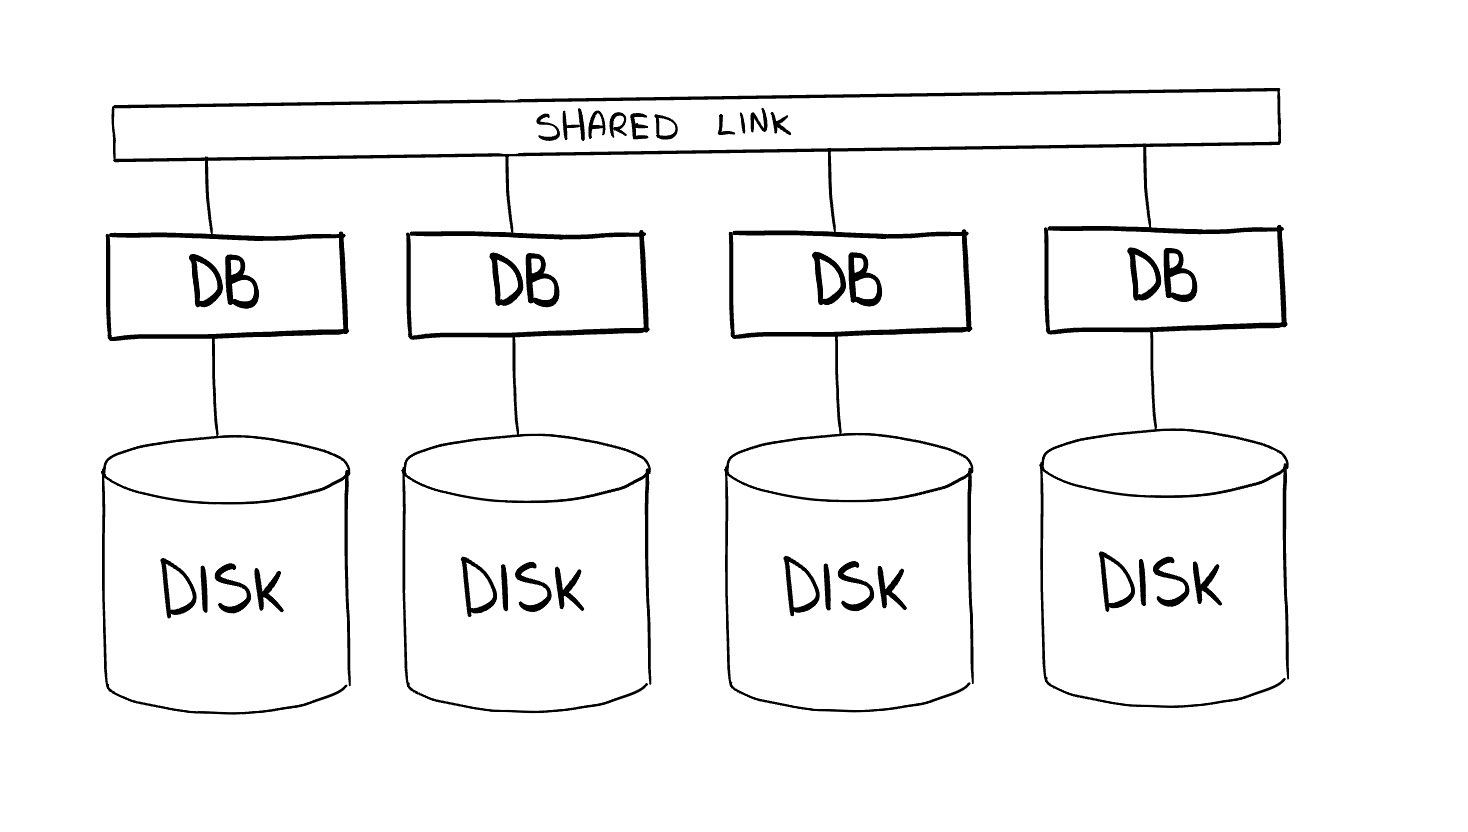
\includegraphics[width=0.60\textwidth]{img/SharedEverything.jpg}
      \caption{Architettura shared-everything}
      \label{fig:sharedEverything}
\end{figure}
Vediamo quindi le proprietà generali di un DDBMS:
\begin{itemize}
    \item \textbf{Località}: i dati sono vicino alle applicazioni che li
          utilizzano più frequentemente. Questo riduce i tempi per l'esecuzione
          delle operazioni. Il paradigma è spostare i dati verso le
          applicazioni, le partizioni dei dati corrispondono spesso a delle
          partizioni naturali delle applicazioni e degli utenti. Le
          distribuzioni dei dati spesso è flessibile: è possibile spostare un
          intera tabella così come è possibile spostarne solo un sottoinsieme
          o replicarla.
    \item \textbf{Modularità} le modifiche alle applicazioni e ai dati possono
          essere effettuate a basso costo.
    \item \textbf{Resistenza ai guasti}: grazie alla replicazione dei dati
    \item \textbf{Prestazioni ed Efficienza}: distribuendo un database su più
          nodi, ogni nodo gestisce un DB di dimensioni ridotte. Questo
          significa che i singoli DB sono più facili da gestire e ottimizzare
          localmente e, in particolare, ogni nodo può adottare delle
          ottimizzazioni personalizzate. Il carico inoltre viene distribuito
          sui nodi. Tutto ciò però richiede chiaramente un coordinamento tra i
          nodi e aumenta il traffico di rete che può rivelarsi un collo di
          bottiglia per le prestazioni.
\end{itemize}

Si hanno le seguenti funzionalità specifiche:
\begin{itemize}
    \item \textbf{Trasmissione} di query, transizioni, frammenti di db e dati
          di controllo tra i nodi.
    \item \textbf{Frammentazione, replicazione e trasparenza} fattori legati
          alla natura distribuita dei dati.
    \item un query processor e un query plan per la previsione di una
          strategia globale accanto a strategie per le query locali. Si gestisce
          il passaggio tra schema logico globale e quelli locali. Chi esegue
          la query lo fa senza pensare alla frammentazione dei dati
    \item \textbf{Controllo di concorrenza} tramite algoritmi distribuiti, fondamentale
          per gli accessi in scrittura.
    \item \textbf{Strategie di recovery} e \textbf{gestione dei guasti}, sia
          in merito alla rete che all'hardware stesso.
\end{itemize}
\subsection{Frammentazione e replicazione}
\begin{definizione}[\textbf{Frammentazione}]
    Si definisce \textbf{frammentazione} come la possibilità di allocare porzioni
    diverse del database su nodi diversi.
\end{definizione}
\begin{definizione}[\textbf{Replicazione}]
    Si definisce \textbf{replicazione} come la possibilità di allocare stesse
    porzioni del database su nodi diversi.
\end{definizione}
\begin{definizione}[\textbf{Trasparenza}]
    Si definisce \textbf{trasparenza} come la possibilità per l'applicazione di
    accedere ai dati senza sapere dove sono allocati.
\end{definizione}
\subsubsection{Frammentazione}
Esistono due tipi di frammentazione:
\begin{itemize}
    \item \textbf{Frammentazione orizzontale}: si prende una tabella e la si
          frammenta in base alle righe. Si mantiene inalterato lo schema in
          quanto si ottengono solo delle tabelle più piccole. Per spezzare si
          usa una select che selezioni ogni volta un certo blocco di tabella.
    \item \textbf{Frammentazione verticale}: si prende una tabella e la si frammenta
          in base alle colonne. In ogni nuova tabella però la prima colonna
          deve essere uguale alla prima della tabella originale (ovvero dove si
          ha la chiave primaria), questo per garantire che si possa ricomporre
          la tabella originale con operazioni di join e garantire la
          trasparenza. Anche in questo caso uso una select che selezioni ogni
          volta un certo numero di colonne da mettere nella nuova tabella.
\end{itemize}
Bisogna garantire:
\begin{itemize}
    \item \textbf{Completezza}: ogni record della relazione R di partenza
          deve poter essere ritrovato in almeno uno dei frammenti
    \item \textbf{Ricostruibilità}: la relazione R di partenza deve poter essere
          ricostruita senza perdita di informazione a partire dai frammenti
    \item \textbf{Disgiunzione}: ogni record della relazione R deve essere
          rappresentato in uno solo dei frammenti
    \item \textbf{Replicazione}: l'opposto della disgiunzione
\end{itemize}
\subsubsection{Replicazione}
Si hanno diversi aspetti positivi per l'accesso in lettura, come il miglioramento
delle prestazioni in quanto consente la coesistenza di applicazioni con requisiti
operazionali diversi sugli stessi dati e aumenta la località dei dati usati da
ogni applicazioni. Nel momento in cui si ha l'accesso in scrittura si hanno però
diversi aspetti negativi. Si hanno diverse complicazioni architetturali, tra cui
la gestione della transazioni e l'update di copie multiple, che devono essere
tutte aggiornate. Inoltre bisogna studiare dal punto di vista progettuale cosa
replicare, quanto replicare, dove allocare le copie e le politiche per gestirle.

In merito all'allocazione studiamo anche gli schemi di allocazione. Ogni
frammento può essere allocato su un nodo diverso. Lo schema globale quindi
è solo virtuale e lo schema di allocazione definisce il mapping tra un frammento
e un nodo. Si ha quindi una tabella, un catalogo, che ci da informazioni sul
partizionamento, associando ogni frammento al nodo in cui è allocato.
\subsubsection{Trasparenza}
Con la trasparenza si ha la separazione della semantica di alto livello dalle
modalità di frammentazione e allocazione. Si separa quindi la logica applicativa
dalla logica dei dati ma per farlo serve uno strato software che gestisca la
traduzione dallo schema unico ai sottoschemi, comportando un aumento di
complessità del sistema e una perdita di prestazioni.
Le applicazioni (transazioni, interrogazioni) non devono essere modificate a
seguito di cambiamenti nella definizione e organizzazione dei dati e si hanno
due tipi di trasparenza, che si applicano agli schemi ANSI-SPARC nel
modello distribuito:
\begin{enumerate}
    \item \textbf{Trasparenza logica} (o indipendenza logica), ovvero indipendenza
          dell'applicazione da modifiche dello schema logico. Un'applicazione
          che usa un frammento non viene modificata se vengono modificati altri
          frammenti
    \item \textbf{Trasparenza fisica} (o indipendenza fisica), ovvero indipendenza
          dell'applicazione da modifiche dello schema fisico
\end{enumerate}

Frammentazione e allocazione sono tra lo schema logico globale e ogni schema
logico locale. Si hanno quindi tre livelli di trasparenza:
\begin{itemize}
    \item \textbf{Trasparenza di frammentazione}, che permette di ignorare
          l'esistenza dei frammenti ed è lo scenario migliore per la programmazione
          applicativa con un'applicazione scritta in SQL standard. Il sistema si
          occupa di convertire query globali in locali e relazioni in sotto-relazioni.
          La scomposizione delle query per ogni sotto-relazione è detta query rewriting
    \item \textbf{Trasparenza di replicazione/allocazione}, dove l'applicazione
          è consapevole dei frammenti ma non dei nodi in cui si trovano. In questo
          caso la query è già spezzata in quanto si sa di avere a che fare con un
          sistema frammentato
    \item \textbf{Trasparenza di linguaggio}, dove l'applicazione specifica sia i
          frammenti che i nodi, nodi che possono offrire interfacce che non sono
          SQL standard. Tuttavia l'applicazione sarà scritta in SQL standard a
          prescindere dai linguaggi locali dei nodi. Le query vengono quindi tradotte
          ottimizzatone di query. Questo è il livello di trasparenza più basso
\end{itemize}
